\documentclass[twoside]{book}

% Packages required by doxygen
\usepackage{fixltx2e}
\usepackage{calc}
\usepackage{doxygen}
\usepackage[export]{adjustbox} % also loads graphicx
\usepackage{graphicx}
\usepackage[utf8]{inputenc}
\usepackage{makeidx}
\usepackage{multicol}
\usepackage{multirow}
\PassOptionsToPackage{warn}{textcomp}
\usepackage{textcomp}
\usepackage[nointegrals]{wasysym}
\usepackage[table]{xcolor}

% Font selection
\usepackage[T1]{fontenc}
\usepackage[scaled=.90]{helvet}
\usepackage{courier}
\usepackage{amssymb}
\usepackage{sectsty}
\renewcommand{\familydefault}{\sfdefault}
\allsectionsfont{%
  \fontseries{bc}\selectfont%
  \color{darkgray}%
}
\renewcommand{\DoxyLabelFont}{%
  \fontseries{bc}\selectfont%
  \color{darkgray}%
}
\newcommand{\+}{\discretionary{\mbox{\scriptsize$\hookleftarrow$}}{}{}}

% Page & text layout
\usepackage{geometry}
\geometry{%
  a4paper,%
  top=2.5cm,%
  bottom=2.5cm,%
  left=2.5cm,%
  right=2.5cm%
}
\tolerance=750
\hfuzz=15pt
\hbadness=750
\setlength{\emergencystretch}{15pt}
\setlength{\parindent}{0cm}
\setlength{\parskip}{3ex plus 2ex minus 2ex}
\makeatletter
\renewcommand{\paragraph}{%
  \@startsection{paragraph}{4}{0ex}{-1.0ex}{1.0ex}{%
    \normalfont\normalsize\bfseries\SS@parafont%
  }%
}
\renewcommand{\subparagraph}{%
  \@startsection{subparagraph}{5}{0ex}{-1.0ex}{1.0ex}{%
    \normalfont\normalsize\bfseries\SS@subparafont%
  }%
}
\makeatother

% Headers & footers
\usepackage{fancyhdr}
\pagestyle{fancyplain}
\fancyhead[LE]{\fancyplain{}{\bfseries\thepage}}
\fancyhead[CE]{\fancyplain{}{}}
\fancyhead[RE]{\fancyplain{}{\bfseries\leftmark}}
\fancyhead[LO]{\fancyplain{}{\bfseries\rightmark}}
\fancyhead[CO]{\fancyplain{}{}}
\fancyhead[RO]{\fancyplain{}{\bfseries\thepage}}
\fancyfoot[LE]{\fancyplain{}{}}
\fancyfoot[CE]{\fancyplain{}{}}
\fancyfoot[RE]{\fancyplain{}{\bfseries\scriptsize Generated by Doxygen }}
\fancyfoot[LO]{\fancyplain{}{\bfseries\scriptsize Generated by Doxygen }}
\fancyfoot[CO]{\fancyplain{}{}}
\fancyfoot[RO]{\fancyplain{}{}}
\renewcommand{\footrulewidth}{0.4pt}
\renewcommand{\chaptermark}[1]{%
  \markboth{#1}{}%
}
\renewcommand{\sectionmark}[1]{%
  \markright{\thesection\ #1}%
}

% Indices & bibliography
\usepackage{natbib}
\usepackage[titles]{tocloft}
\setcounter{tocdepth}{3}
\setcounter{secnumdepth}{5}
\makeindex

% Hyperlinks (required, but should be loaded last)
\usepackage{ifpdf}
\ifpdf
  \usepackage[pdftex,pagebackref=true]{hyperref}
\else
  \usepackage[ps2pdf,pagebackref=true]{hyperref}
\fi
\hypersetup{%
  colorlinks=true,%
  linkcolor=blue,%
  citecolor=blue,%
  unicode%
}

% Custom commands
\newcommand{\clearemptydoublepage}{%
  \newpage{\pagestyle{empty}\cleardoublepage}%
}

\usepackage{caption}
\captionsetup{labelsep=space,justification=centering,font={bf},singlelinecheck=off,skip=4pt,position=top}

%===== C O N T E N T S =====

\begin{document}

% Titlepage & ToC
\hypersetup{pageanchor=false,
             bookmarksnumbered=true,
             pdfencoding=unicode
            }
\pagenumbering{alph}
\begin{titlepage}
\vspace*{7cm}
\begin{center}%
{\Large My Project }\\
\vspace*{1cm}
{\large Generated by Doxygen 1.8.13}\\
\end{center}
\end{titlepage}
\clearemptydoublepage
\pagenumbering{roman}
\tableofcontents
\clearemptydoublepage
\pagenumbering{arabic}
\hypersetup{pageanchor=true}

%--- Begin generated contents ---
\chapter{Class Index}
\section{Class List}
Here are the classes, structs, unions and interfaces with brief descriptions\+:\begin{DoxyCompactList}
\item\contentsline{section}{\hyperlink{classDFA}{D\+FA} }{\pageref{classDFA}}{}
\item\contentsline{section}{\hyperlink{classGrammar}{Grammar} }{\pageref{classGrammar}}{}
\item\contentsline{section}{\hyperlink{classIOFile}{I\+O\+File} }{\pageref{classIOFile}}{}
\item\contentsline{section}{\hyperlink{classProduccion}{Produccion} }{\pageref{classProduccion}}{}
\item\contentsline{section}{\hyperlink{classSet}{Set} }{\pageref{classSet}}{}
\item\contentsline{section}{\hyperlink{classTransition}{Transition} }{\pageref{classTransition}}{}
\end{DoxyCompactList}

\chapter{Class Documentation}
\hypertarget{classDFA}{}\section{D\+FA Class Reference}
\label{classDFA}\index{D\+FA@{D\+FA}}
\subsection*{Public Member Functions}
\begin{DoxyCompactItemize}
\item 
\mbox{\Hypertarget{classDFA_a69571967ef142033f6794ef249bc6b3a}\label{classDFA_a69571967ef142033f6794ef249bc6b3a}} 
{\bfseries D\+FA} (std\+::string, std\+::string)
\end{DoxyCompactItemize}


The documentation for this class was generated from the following files\+:\begin{DoxyCompactItemize}
\item 
D\+F\+A.\+h\item 
D\+F\+A.\+cc\end{DoxyCompactItemize}

\hypertarget{classGrammar}{}\section{Grammar Class Reference}
\label{classGrammar}\index{Grammar@{Grammar}}
\subsection*{Public Member Functions}
\begin{DoxyCompactItemize}
\item 
\hyperlink{classGrammar_aa201250a002a7d07d398fee189a74427}{Grammar} ()
\item 
\mbox{\Hypertarget{classGrammar_ac0e288917edf6689b09ba7066ec24b96}\label{classGrammar_ac0e288917edf6689b09ba7066ec24b96}} 
void {\bfseries Set\+Alphabet} (std\+::set$<$ std\+::string $>$)
\item 
\mbox{\Hypertarget{classGrammar_ae9e0c4be302e137bc2587c487d7c4b6a}\label{classGrammar_ae9e0c4be302e137bc2587c487d7c4b6a}} 
void {\bfseries Set\+States} (std\+::set$<$ std\+::string $>$)
\item 
void \hyperlink{classGrammar_a8729a9cee27c29079970a78163c8ed0f}{Set\+Start} (std\+::string)
\item 
void \hyperlink{classGrammar_a182676fa0ce7f6ce737a2fd4c357b3e2}{Set\+Accept\+States} (std\+::set$<$ std\+::string $>$)
\item 
\mbox{\Hypertarget{classGrammar_a6bba075a6a8c00f3cd5182deb15e9290}\label{classGrammar_a6bba075a6a8c00f3cd5182deb15e9290}} 
void {\bfseries Set\+Produccion} (std\+::string, std\+::string, std\+::string)
\item 
void \hyperlink{classGrammar_a4bb28fac57fe1177d5e95e833d3717d1}{Print\+File} (std\+::string)
\end{DoxyCompactItemize}


\subsection{Constructor \& Destructor Documentation}
\mbox{\Hypertarget{classGrammar_aa201250a002a7d07d398fee189a74427}\label{classGrammar_aa201250a002a7d07d398fee189a74427}} 
\index{Grammar@{Grammar}!Grammar@{Grammar}}
\index{Grammar@{Grammar}!Grammar@{Grammar}}
\subsubsection{\texorpdfstring{Grammar()}{Grammar()}}
{\footnotesize\ttfamily Grammar\+::\+Grammar (\begin{DoxyParamCaption}{ }\end{DoxyParamCaption})}

we set the bools to false as init 

\subsection{Member Function Documentation}
\mbox{\Hypertarget{classGrammar_a4bb28fac57fe1177d5e95e833d3717d1}\label{classGrammar_a4bb28fac57fe1177d5e95e833d3717d1}} 
\index{Grammar@{Grammar}!Print\+File@{Print\+File}}
\index{Print\+File@{Print\+File}!Grammar@{Grammar}}
\subsubsection{\texorpdfstring{Print\+File()}{PrintFile()}}
{\footnotesize\ttfamily void Grammar\+::\+Print\+File (\begin{DoxyParamCaption}\item[{std\+::string}]{output\+\_\+file }\end{DoxyParamCaption})}

we open the output file and write the result in it \mbox{\Hypertarget{classGrammar_a182676fa0ce7f6ce737a2fd4c357b3e2}\label{classGrammar_a182676fa0ce7f6ce737a2fd4c357b3e2}} 
\index{Grammar@{Grammar}!Set\+Accept\+States@{Set\+Accept\+States}}
\index{Set\+Accept\+States@{Set\+Accept\+States}!Grammar@{Grammar}}
\subsubsection{\texorpdfstring{Set\+Accept\+States()}{SetAcceptStates()}}
{\footnotesize\ttfamily void Grammar\+::\+Set\+Accept\+States (\begin{DoxyParamCaption}\item[{std\+::set$<$ std\+::string $>$}]{set\+\_\+state }\end{DoxyParamCaption})}

if start state belong to the set of states, we add it \mbox{\Hypertarget{classGrammar_a8729a9cee27c29079970a78163c8ed0f}\label{classGrammar_a8729a9cee27c29079970a78163c8ed0f}} 
\index{Grammar@{Grammar}!Set\+Start@{Set\+Start}}
\index{Set\+Start@{Set\+Start}!Grammar@{Grammar}}
\subsubsection{\texorpdfstring{Set\+Start()}{SetStart()}}
{\footnotesize\ttfamily void Grammar\+::\+Set\+Start (\begin{DoxyParamCaption}\item[{std\+::string}]{start }\end{DoxyParamCaption})}

if start state belong to state, we add it 

The documentation for this class was generated from the following files\+:\begin{DoxyCompactItemize}
\item 
Grammar.\+h\item 
Grammar.\+cc\end{DoxyCompactItemize}

\hypertarget{classIOFile}{}\section{I\+O\+File Class Reference}
\label{classIOFile}\index{I\+O\+File@{I\+O\+File}}


Collaboration diagram for I\+O\+File\+:
\nopagebreak
\begin{figure}[H]
\begin{center}
\leavevmode
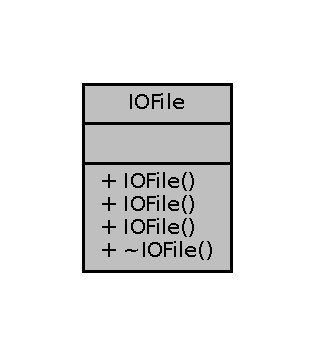
\includegraphics[width=151pt]{classIOFile__coll__graph}
\end{center}
\end{figure}
\subsection*{Public Member Functions}
\begin{DoxyCompactItemize}
\item 
\hyperlink{classIOFile_a1a08441371c84205a8704c6ef0811792}{I\+O\+File} (std\+::string, std\+::string)
\item 
\hyperlink{classIOFile_a25f35de90baaae5b5b8553802285806b}{I\+O\+File} (std\+::string, std\+::string, std\+::string)
\end{DoxyCompactItemize}


\subsection{Constructor \& Destructor Documentation}
\mbox{\Hypertarget{classIOFile_a1a08441371c84205a8704c6ef0811792}\label{classIOFile_a1a08441371c84205a8704c6ef0811792}} 
\index{I\+O\+File@{I\+O\+File}!I\+O\+File@{I\+O\+File}}
\index{I\+O\+File@{I\+O\+File}!I\+O\+File@{I\+O\+File}}
\subsubsection{\texorpdfstring{I\+O\+File()}{IOFile()}\hspace{0.1cm}{\footnotesize\ttfamily [1/2]}}
{\footnotesize\ttfamily I\+O\+File\+::\+I\+O\+File (\begin{DoxyParamCaption}\item[{std\+::string}]{input,  }\item[{std\+::string}]{output }\end{DoxyParamCaption})}

Constructor of P5 \mbox{\Hypertarget{classIOFile_a25f35de90baaae5b5b8553802285806b}\label{classIOFile_a25f35de90baaae5b5b8553802285806b}} 
\index{I\+O\+File@{I\+O\+File}!I\+O\+File@{I\+O\+File}}
\index{I\+O\+File@{I\+O\+File}!I\+O\+File@{I\+O\+File}}
\subsubsection{\texorpdfstring{I\+O\+File()}{IOFile()}\hspace{0.1cm}{\footnotesize\ttfamily [2/2]}}
{\footnotesize\ttfamily I\+O\+File\+::\+I\+O\+File (\begin{DoxyParamCaption}\item[{std\+::string}]{pattern,  }\item[{std\+::string}]{input,  }\item[{std\+::string}]{output }\end{DoxyParamCaption})}

Constructor of P6 

The documentation for this class was generated from the following files\+:\begin{DoxyCompactItemize}
\item 
Iofile.\+h\item 
Iofile.\+cc\end{DoxyCompactItemize}

\hypertarget{classProduccion}{}\section{Produccion Class Reference}
\label{classProduccion}\index{Produccion@{Produccion}}
\subsection*{Public Member Functions}
\begin{DoxyCompactItemize}
\item 
void \hyperlink{classProduccion_a7ddb6e615717aefd0f2ed7882dab617f}{Clear\+Produccion} (void)
\item 
void \hyperlink{classProduccion_a5b6a6304f6984b2247dc52707b50d51d}{Insert} (std\+::string, std\+::string, std\+::string)
\item 
\mbox{\Hypertarget{classProduccion_aac707505e20c194e315d032b97db363e}\label{classProduccion_aac707505e20c194e315d032b97db363e}} 
int {\bfseries Get\+Size} (void)
\item 
\mbox{\Hypertarget{classProduccion_a4f5cbc7f7b2203dcafffb481fbaa8d56}\label{classProduccion_a4f5cbc7f7b2203dcafffb481fbaa8d56}} 
Node $\ast$ {\bfseries Get\+Node} (int position)
\end{DoxyCompactItemize}


\subsection{Member Function Documentation}
\mbox{\Hypertarget{classProduccion_a7ddb6e615717aefd0f2ed7882dab617f}\label{classProduccion_a7ddb6e615717aefd0f2ed7882dab617f}} 
\index{Produccion@{Produccion}!Clear\+Produccion@{Clear\+Produccion}}
\index{Clear\+Produccion@{Clear\+Produccion}!Produccion@{Produccion}}
\subsubsection{\texorpdfstring{Clear\+Produccion()}{ClearProduccion()}}
{\footnotesize\ttfamily void Produccion\+::\+Clear\+Produccion (\begin{DoxyParamCaption}\item[{void}]{ }\end{DoxyParamCaption})}

we erase the duplicates productions \mbox{\Hypertarget{classProduccion_a5b6a6304f6984b2247dc52707b50d51d}\label{classProduccion_a5b6a6304f6984b2247dc52707b50d51d}} 
\index{Produccion@{Produccion}!Insert@{Insert}}
\index{Insert@{Insert}!Produccion@{Produccion}}
\subsubsection{\texorpdfstring{Insert()}{Insert()}}
{\footnotesize\ttfamily void Produccion\+::\+Insert (\begin{DoxyParamCaption}\item[{std\+::string}]{initstate,  }\item[{std\+::string}]{symbol,  }\item[{std\+::string}]{finalstate }\end{DoxyParamCaption})}

we insert the production in the vector 

The documentation for this class was generated from the following files\+:\begin{DoxyCompactItemize}
\item 
Produccion.\+h\item 
Produccion.\+cc\end{DoxyCompactItemize}

\hypertarget{classSet}{}\section{Set Class Reference}
\label{classSet}\index{Set@{Set}}
\subsection*{Public Member Functions}
\begin{DoxyCompactItemize}
\item 
\mbox{\Hypertarget{classSet_a545e44270dff7f873f7203aa5c6ca3a1}\label{classSet_a545e44270dff7f873f7203aa5c6ca3a1}} 
{\bfseries Set} (int)
\item 
\mbox{\Hypertarget{classSet_a9387dcd9189f0b036d731cf4f169de05}\label{classSet_a9387dcd9189f0b036d731cf4f169de05}} 
{\bfseries Set} (std\+::string, std\+::string)
\item 
void \hyperlink{classSet_aa25ad5b9d72e4d428eb564b2eb208e3b}{Work} (std\+::string)
\item 
\mbox{\Hypertarget{classSet_acc57a5a86498c7efb365b4dfbf1fd247}\label{classSet_acc57a5a86498c7efb365b4dfbf1fd247}} 
void {\bfseries Set\+Output} (std\+::ofstream \&)
\item 
std\+::string \hyperlink{classSet_afc0f35a8d6903b892bb283813511fea9}{Write} ()
\item 
\mbox{\Hypertarget{classSet_af72ca387c44c1768ec7c7ec4e9a94f37}\label{classSet_af72ca387c44c1768ec7c7ec4e9a94f37}} 
void {\bfseries Save\+Result} (std\+::string)
\item 
\mbox{\Hypertarget{classSet_afa9c6e6f6b0dedc1a397a0f8a85fc3a6}\label{classSet_afa9c6e6f6b0dedc1a397a0f8a85fc3a6}} 
std\+::string {\bfseries Get\+Result} ()
\item 
void \hyperlink{classSet_abe5c5439f3665baba2da0b1f1a4c03fd}{Clear} ()
\item 
bool \hyperlink{classSet_a0361a3a2b7a408514a259b326245cbc7}{Is\+Empty} ()
\item 
bool \hyperlink{classSet_a8fb9899afe9a09628706cf539cc75a1c}{Belong} (int)
\item 
void \hyperlink{classSet_a7f28cadb13f4cc86a87f64b9f885877a}{operator=} (std\+::string)
\item 
bool \hyperlink{classSet_a3087ba7a27e33fbb1b2a091c405ba046}{operator==} (\hyperlink{classSet}{Set})
\item 
void \hyperlink{classSet_a33786bba5f634c5023d047b5f1f1a292}{operator+} (int)
\item 
void \hyperlink{classSet_a1e58afdc9befac1dbe295a0bdccfeacb}{operator-\/} (int)
\item 
\mbox{\Hypertarget{classSet_a1440c7bdad66b1864b41b4aafb188245}\label{classSet_a1440c7bdad66b1864b41b4aafb188245}} 
void {\bfseries Print\+Set} (void)
\item 
void \hyperlink{classSet_a167b6d87b1698a61f269835c34c455cc}{Print\+Vector\+Set} (std\+::vector$<$ unsigned long int $>$)
\item 
\mbox{\Hypertarget{classSet_a6c55977d6e5c48ab791bbe49e832c5ba}\label{classSet_a6c55977d6e5c48ab791bbe49e832c5ba}} 
int {\bfseries Get\+Size\+Of\+Set} (void)
\item 
void \hyperlink{classSet_abd4f422aa428bed3afba157f4a18c90f}{Set\+Alphabet} (std\+::string)
\item 
\mbox{\Hypertarget{classSet_acd8545ba5646eb4be510a19a17dd78e4}\label{classSet_acd8545ba5646eb4be510a19a17dd78e4}} 
void {\bfseries Set\+States} (std\+::string)
\item 
bool \hyperlink{classSet_a80ff19b9d44830084708478bac29231b}{Belong\+Alpha} (std\+::string)
\item 
bool \hyperlink{classSet_a8300b84ddc30a216c3e2d1b467e606bc}{Belong\+States} (std\+::string)
\end{DoxyCompactItemize}
\subsection*{Public Attributes}
\begin{DoxyCompactItemize}
\item 
\mbox{\Hypertarget{classSet_a22a8ef647115a534ffba7bac30e44676}\label{classSet_a22a8ef647115a534ffba7bac30e44676}} 
int {\bfseries size\+\_\+of\+\_\+set\+\_\+}
\item 
\mbox{\Hypertarget{classSet_a9c6f21f89012e343006db3672289728d}\label{classSet_a9c6f21f89012e343006db3672289728d}} 
int {\bfseries counter\+\_\+mod\+\_\+}
\end{DoxyCompactItemize}


\subsection{Member Function Documentation}
\mbox{\Hypertarget{classSet_a8fb9899afe9a09628706cf539cc75a1c}\label{classSet_a8fb9899afe9a09628706cf539cc75a1c}} 
\index{Set@{Set}!Belong@{Belong}}
\index{Belong@{Belong}!Set@{Set}}
\subsubsection{\texorpdfstring{Belong()}{Belong()}}
{\footnotesize\ttfamily bool Set\+::\+Belong (\begin{DoxyParamCaption}\item[{int}]{number }\end{DoxyParamCaption})}

return true if the element belong to the set \mbox{\Hypertarget{classSet_a80ff19b9d44830084708478bac29231b}\label{classSet_a80ff19b9d44830084708478bac29231b}} 
\index{Set@{Set}!Belong\+Alpha@{Belong\+Alpha}}
\index{Belong\+Alpha@{Belong\+Alpha}!Set@{Set}}
\subsubsection{\texorpdfstring{Belong\+Alpha()}{BelongAlpha()}}
{\footnotesize\ttfamily bool Set\+::\+Belong\+Alpha (\begin{DoxyParamCaption}\item[{std\+::string}]{alpha }\end{DoxyParamCaption})}

return true if alpha belong to the set of alpha \mbox{\Hypertarget{classSet_a8300b84ddc30a216c3e2d1b467e606bc}\label{classSet_a8300b84ddc30a216c3e2d1b467e606bc}} 
\index{Set@{Set}!Belong\+States@{Belong\+States}}
\index{Belong\+States@{Belong\+States}!Set@{Set}}
\subsubsection{\texorpdfstring{Belong\+States()}{BelongStates()}}
{\footnotesize\ttfamily bool Set\+::\+Belong\+States (\begin{DoxyParamCaption}\item[{std\+::string}]{alpha }\end{DoxyParamCaption})}

return true if the state belong to the set of state \mbox{\Hypertarget{classSet_abe5c5439f3665baba2da0b1f1a4c03fd}\label{classSet_abe5c5439f3665baba2da0b1f1a4c03fd}} 
\index{Set@{Set}!Clear@{Clear}}
\index{Clear@{Clear}!Set@{Set}}
\subsubsection{\texorpdfstring{Clear()}{Clear()}}
{\footnotesize\ttfamily void Set\+::\+Clear (\begin{DoxyParamCaption}{ }\end{DoxyParamCaption})}

clear the set \mbox{\Hypertarget{classSet_a0361a3a2b7a408514a259b326245cbc7}\label{classSet_a0361a3a2b7a408514a259b326245cbc7}} 
\index{Set@{Set}!Is\+Empty@{Is\+Empty}}
\index{Is\+Empty@{Is\+Empty}!Set@{Set}}
\subsubsection{\texorpdfstring{Is\+Empty()}{IsEmpty()}}
{\footnotesize\ttfamily bool Set\+::\+Is\+Empty (\begin{DoxyParamCaption}{ }\end{DoxyParamCaption})}

return true if set is empty \mbox{\Hypertarget{classSet_a33786bba5f634c5023d047b5f1f1a292}\label{classSet_a33786bba5f634c5023d047b5f1f1a292}} 
\index{Set@{Set}!operator+@{operator+}}
\index{operator+@{operator+}!Set@{Set}}
\subsubsection{\texorpdfstring{operator+()}{operator+()}}
{\footnotesize\ttfamily void Set\+::operator+ (\begin{DoxyParamCaption}\item[{int}]{sum }\end{DoxyParamCaption})}

overload of + \mbox{\Hypertarget{classSet_a1e58afdc9befac1dbe295a0bdccfeacb}\label{classSet_a1e58afdc9befac1dbe295a0bdccfeacb}} 
\index{Set@{Set}!operator-\/@{operator-\/}}
\index{operator-\/@{operator-\/}!Set@{Set}}
\subsubsection{\texorpdfstring{operator-\/()}{operator-()}}
{\footnotesize\ttfamily void Set\+::operator-\/ (\begin{DoxyParamCaption}\item[{int}]{sum }\end{DoxyParamCaption})}

overload of -\/ \mbox{\Hypertarget{classSet_a7f28cadb13f4cc86a87f64b9f885877a}\label{classSet_a7f28cadb13f4cc86a87f64b9f885877a}} 
\index{Set@{Set}!operator=@{operator=}}
\index{operator=@{operator=}!Set@{Set}}
\subsubsection{\texorpdfstring{operator=()}{operator=()}}
{\footnotesize\ttfamily void Set\+::operator= (\begin{DoxyParamCaption}\item[{std\+::string}]{in }\end{DoxyParamCaption})}

overload of = \mbox{\Hypertarget{classSet_a3087ba7a27e33fbb1b2a091c405ba046}\label{classSet_a3087ba7a27e33fbb1b2a091c405ba046}} 
\index{Set@{Set}!operator==@{operator==}}
\index{operator==@{operator==}!Set@{Set}}
\subsubsection{\texorpdfstring{operator==()}{operator==()}}
{\footnotesize\ttfamily bool Set\+::operator== (\begin{DoxyParamCaption}\item[{\hyperlink{classSet}{Set}}]{in }\end{DoxyParamCaption})}

overload of == \mbox{\Hypertarget{classSet_a167b6d87b1698a61f269835c34c455cc}\label{classSet_a167b6d87b1698a61f269835c34c455cc}} 
\index{Set@{Set}!Print\+Vector\+Set@{Print\+Vector\+Set}}
\index{Print\+Vector\+Set@{Print\+Vector\+Set}!Set@{Set}}
\subsubsection{\texorpdfstring{Print\+Vector\+Set()}{PrintVectorSet()}}
{\footnotesize\ttfamily void Set\+::\+Print\+Vector\+Set (\begin{DoxyParamCaption}\item[{std\+::vector$<$ unsigned long int $>$}]{data }\end{DoxyParamCaption})}

prints all the bits of the vector \mbox{\Hypertarget{classSet_abd4f422aa428bed3afba157f4a18c90f}\label{classSet_abd4f422aa428bed3afba157f4a18c90f}} 
\index{Set@{Set}!Set\+Alphabet@{Set\+Alphabet}}
\index{Set\+Alphabet@{Set\+Alphabet}!Set@{Set}}
\subsubsection{\texorpdfstring{Set\+Alphabet()}{SetAlphabet()}}
{\footnotesize\ttfamily void Set\+::\+Set\+Alphabet (\begin{DoxyParamCaption}\item[{std\+::string}]{alpha\+\_\+char }\end{DoxyParamCaption})}

we set here the alphabet \mbox{\Hypertarget{classSet_aa25ad5b9d72e4d428eb564b2eb208e3b}\label{classSet_aa25ad5b9d72e4d428eb564b2eb208e3b}} 
\index{Set@{Set}!Work@{Work}}
\index{Work@{Work}!Set@{Set}}
\subsubsection{\texorpdfstring{Work()}{Work()}}
{\footnotesize\ttfamily void Set\+::\+Work (\begin{DoxyParamCaption}\item[{std\+::string}]{in }\end{DoxyParamCaption})}

calling private functions for make the class work. \mbox{\Hypertarget{classSet_afc0f35a8d6903b892bb283813511fea9}\label{classSet_afc0f35a8d6903b892bb283813511fea9}} 
\index{Set@{Set}!Write@{Write}}
\index{Write@{Write}!Set@{Set}}
\subsubsection{\texorpdfstring{Write()}{Write()}}
{\footnotesize\ttfamily std\+::string Set\+::\+Write (\begin{DoxyParamCaption}{ }\end{DoxyParamCaption})}

writting the result to the file 

The documentation for this class was generated from the following files\+:\begin{DoxyCompactItemize}
\item 
Set.\+h\item 
Set.\+cc\end{DoxyCompactItemize}

\hypertarget{classTransition}{}\section{Transition Class Reference}
\label{classTransition}\index{Transition@{Transition}}
\subsection*{Public Member Functions}
\begin{DoxyCompactItemize}
\item 
\mbox{\Hypertarget{classTransition_abf32adbb5c39d5a69f8540620f5e2e8c}\label{classTransition_abf32adbb5c39d5a69f8540620f5e2e8c}} 
std\+::string {\bfseries Get\+Final\+Node} (std\+::string, std\+::string)
\item 
\mbox{\Hypertarget{classTransition_adc99d2c2e431cb989e34abea83f71377}\label{classTransition_adc99d2c2e431cb989e34abea83f71377}} 
void {\bfseries Insert} (std\+::string \&, std\+::string \&, std\+::string \&)
\item 
\mbox{\Hypertarget{classTransition_a2f19d29c76337e2b65be2b3a46719963}\label{classTransition_a2f19d29c76337e2b65be2b3a46719963}} 
int {\bfseries Get\+Size} (void)
\item 
\mbox{\Hypertarget{classTransition_a740aa42116d5264e2c16dd7a20a833cf}\label{classTransition_a740aa42116d5264e2c16dd7a20a833cf}} 
Node $\ast$ {\bfseries Get\+Node} (int position)
\end{DoxyCompactItemize}


The documentation for this class was generated from the following files\+:\begin{DoxyCompactItemize}
\item 
Transition.\+h\item 
Transition.\+cc\end{DoxyCompactItemize}

%--- End generated contents ---

% Index
\backmatter
\newpage
\phantomsection
\clearemptydoublepage
\addcontentsline{toc}{chapter}{Index}
\printindex

\end{document}
